\chapter{Introduction}

\section{History}

Fast radio bursts or FRBs, are bright, broadband pulses of radio emission ranging from milliseconds or less, first discovered while reviewing data in radio pulsar surveys \cite{Lorimer2007}. The single pulse (FRB 010724) was detected in a Small Magellanic Cloud survey with the Parkes Telescope in 2001, and had a peak flux density of over 30 Jy and a large dispersive measure, suggesting the existence of a population of bright, extragalactic radio pulses. 

\begin{figure}
    \centering
    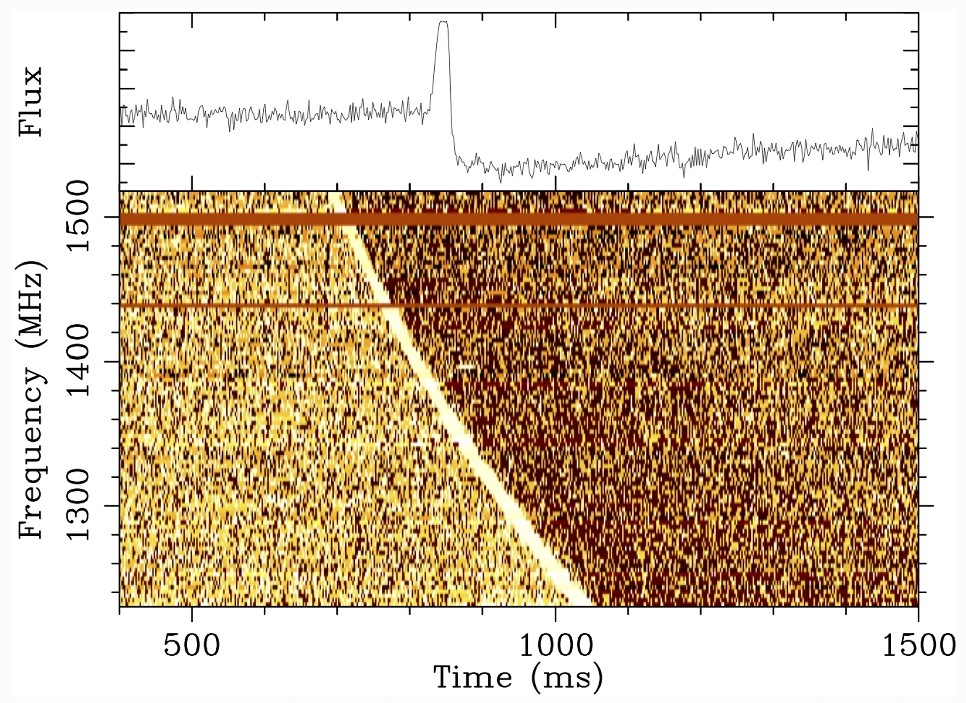
\includegraphics[width=0.65\textwidth]{Images/lorimer.jpg}
    \caption[Lorimer burst]{Frequency spectrum (bottom panel) and integrated pulse shape (top panel) of the Lorimer burst, the first FRB detected using the Parkes Telescope \protect\cite{Lorimer2007}.}
    \label{fig:lorimer}
\end{figure}

This was further strengthened by the detection of four high-dispersion signals in the High Time Resolution Universe survey using the same telescope \cite{Keith2010}. This led to increased searches in new and archived data from the Parkes Telescope, as well as other telescopes such as the Arecibo Telescope \cite{Spitler2014}, the Green Bank Telescope \cite{Masui2015}, the Upgraded Molongo Synthesis Telescope (UTMOST, \citeNP{Caleb2016}), and the Australian Square Kilometre Array Pathfinder (ASKAP, \cite{Bannister2017}). 

\section{Properties of FRBs}

FRBs have flux densities around 50 mJy - 100 Jy with widths between 0.8 ms - 5000 ms. There are currrently 309 FRB detections so far (Transient Name Server\footnote{Transient Name Server (TNS): \url{https://www.wis-tns.org/}} and FRBCAT\footnote{FRBCAT: \url{http://frbcat.org/}}) between frequencies 400 MHz to 8 GHz, and 60\% of them exhibit repeating patterns e.g. FRB 121102 where a periodicity of 161 days was detected \cite{Cruces2020}. A distinct characteristic of FRBs is their frequency-dependent signal delay which follows the cold-plasma dispersion relation. Dispersion is due to the frequency dependent group velocity of a wave packet when propagating in a dispersive medium. The temporal delay in the FRB signal between two frequencies is given by 
\begin{equation} \label{eq:dmdelay}
    t = 4.149 \times \text{DM} \left(\nu_{1,\text{GHz}}^{-2} - \nu_{2,\text{GHz}}^{-2}\right) \text{ms},
\end{equation}
where the dispersion measure (DM) is the column density of free electrons along the line of sight in the unit $\cmp$ i.e. $\text{DM}\equiv\int n_e\,dl$ where $n_e$ is the electron density. The DM values observed from FRBs usually exceed the contribution from our galaxy with FRB 160102 having the largest at $\text{DM} = 2596.1 \pm 0.3 \cmp$ \cite{Petroff_Hessels_Lorimer_2019}.

\begin{figure}
    \centering
    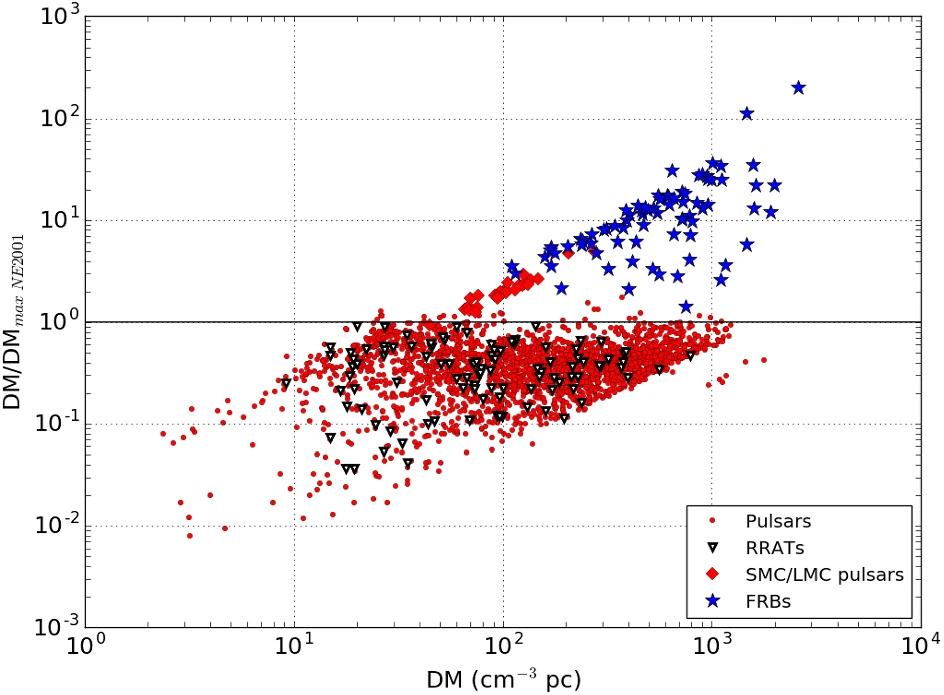
\includegraphics[width=0.7\textwidth]{Images/DM.jpg}
    \caption[DMs of FRBs, RRATs, Pulsars]{Plot of the ratio between the DMs of FRBs, galactic rotating radio transients, pulsars in the Small and Large Magellanic Clouds, and galactic radio pulsars with respect to Milky Way contribution versus their DMs \protect\cite{Petroff_Hessels_Lorimer_2019}.}
    \label{fig:dmdist}
\end{figure}

Another characteristic of FRBs are their polarization, and although only a number of them have polarimetric data, results are mixed i.e. some are unpolarized, some either circularly or linearly polarized, and others have both. Linear polarization is parameterized by Faraday rotation measure, RM and from this, the line-of sight magnetic field strength can be obtained, and the results seem close to that of magnetars \cite{Wang2020}. Various other papers have also pointed the origin of several FRBs to the magnetosphere of magnetars \cite{Luo2020,chime2020} and the current sample of localized FRB hosts is consistent with magnetar progenitors \cite{Bochenek2021}. Magnetars are neutron stars with extremely powerful magnetic fields, up to $10^{15}\,\text{G}$. This points to the `Decelerating Blast Waves in Magnetars' model as the FRB progenitor. 

\section{Progenitor and Emission Theories}

As stated by \citeA{Lyubarsky2014}, relativistic blast waves are emitted when restructuring of the magnetar's core distorts its magnetic field, and the emission is modelled by the synchrotron maser blastwave model, where the blast waves encounter the magnetar's staionary outer shell, causing forward and reverse shocks \cite{Metzger2019}. The reverse shocks moves the shell and produce coherent synchrotron radiation, which is seen as an FRB, whereas the forward shocks produce an x-ray afterglow, as detected in some multi-wavelength FRB observations \cite{Metzger2020}. 

\begin{figure}
    \centering
    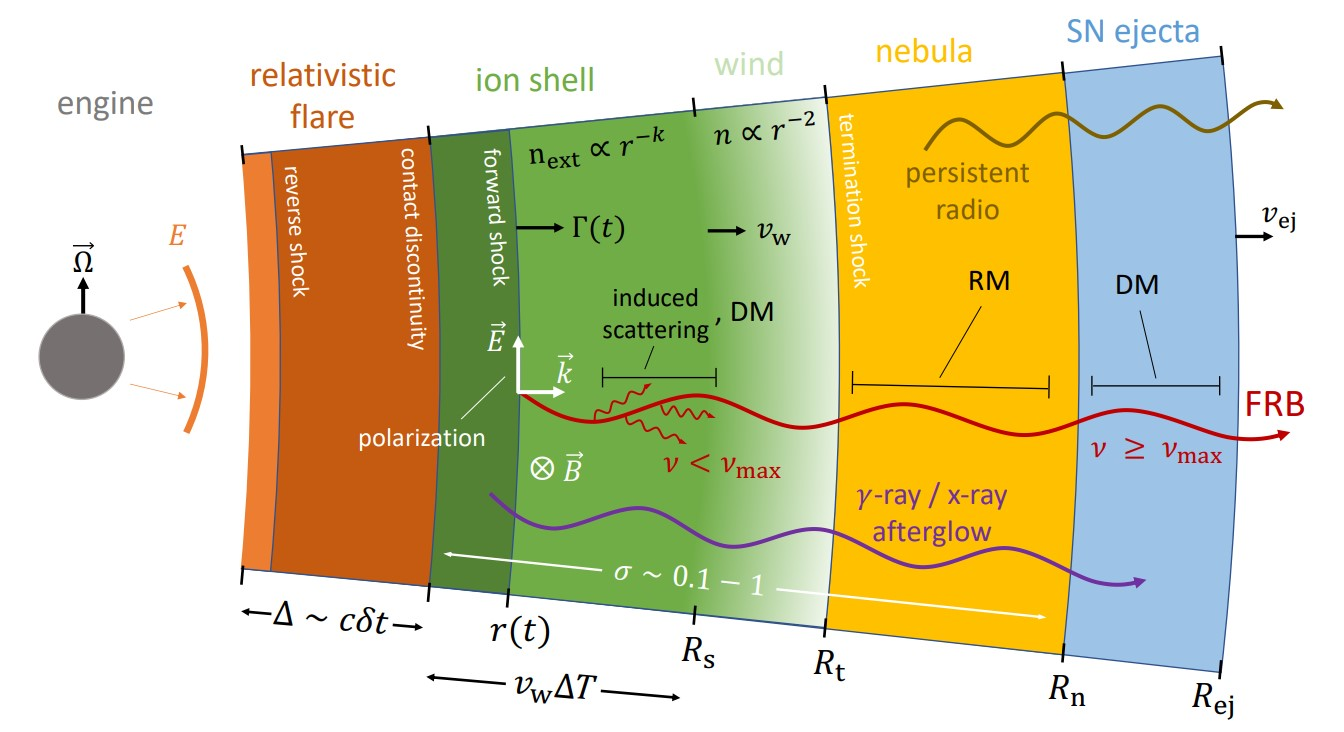
\includegraphics[width=0.9\textwidth]{Images/magnetarprog.jpg}
    \caption[FRB synchrotron maser emission]{Schematic of the production of FRBs as synchrotron maser emission from decelerating relativistic blast waves in magnetars \protect\cite{Metzger2019}.}
    \label{fig:prog}
\end{figure}

Other progenitor theories include mergers such as binary black hole mergers \cite{Zhang2016}, collapses such as dark matter-induced neutron star collapse \cite{Totani2013}, interactions such as neutron star-asteroid belt interaction \cite{Dai2016} and theories involving pulsars such as pulsar wind bubbles \cite{Murase2016}. However, all these theories are purely derived from observational basis and are not confirmed. More FRB observational improvements in terms of higher accuracy, multi-wavelength observations and particle detection could narrow it down on the correct theory for FRBs. 

\section{Astrophyiscal Applications}

Aside from searching for the progenitor of FRBs, FRBs also have other significant astrophysical and/or cosmological applications. Examples include:
\begin{itemize}
    \item Measurement of the Hubble constant via the distance constraint and redshift relation of FRBs \cite{Steffen2021}
    \item Testing of Einstein's equivalence principle from the time delay experienced by photons \cite{Wei2015,Reischke2021}
    \item Bounding of photon rest mass using kinematic analysis of light propagation \cite{Wu2016,Wang2021}
    \item Contraining the epoch of reionization using highly dispersed FRBs \cite{Pagano2021}
    \item Revealing hidden baryons in the Universe using dispersion of localized FRBs \cite{Macquart2020}
    \item Constraining the equation of state of dark energy and other cosmological parameters using DM-redshift relation \cite{Zhou2014}
    \item Measurement of turbulence of cosmic web/intergalactic medium (IGM) from polarization measurements \cite{Ravi2016}
    \item Reconstruction of baryon fraction in the IGM from DM angular power spectrum \cite{Dai2021}
    \item Constraining galaxy haloes using dispersion and scattering of FRBs \cite{Ocker2021}
\end{itemize}

\section{Objectives}

The objectives of this project are:
\begin{itemize}
    \item To understand FRB detection methods
    \item To develop a program that independently searches for FRBs in radio telescope data
    \item To compare performance of the program developed with BEAR
    \item To test the performance increase for GPU dedispersion 
\end{itemize}

This thesis is organized in the following manner. Chapter \ref{litrev} looks at literature on available FRB detection methods, data analysis, and instrumentation involved. Chapter \ref{method} briefs on the flow of the project and explains the methodology involved in the program as well as testing methods. Chapter \ref{result} presents the results of the test. In Chapter \ref{discuss}, discussions regarding the program's performance is made. Finally, the summary of this project is described in Chapter \ref{summary}.